\documentclass[twoside]{thesis_style/upmthesis}
\usepackage{appendix}
\usepackage{listings}

\usepackage{amsmath, amssymb, latexsym}
\usepackage{graphics,epsfig,epsf,rotating,subfigure}
\usepackage{theorem,url,multirow}
\usepackage{rotfloat,array,pifont}
\usepackage{float}


\usepackage[table,usenames,dvipsnames]{xcolor}
\usepackage{lscape}
\usepackage[perpage]{footmisc}
\usepackage[spanish]{babel}
\usepackage{color}
\definecolor{lightgray}{rgb}{.9,.9,.9}
\definecolor{darkgray}{rgb}{.4,.4,.4}
\definecolor{purple}{rgb}{0.65, 0.12, 0.82}
\usepackage{graphicx}
\usepackage{chngcntr}
\counterwithout{figure}{chapter}
\counterwithout{table}{chapter}
\lstdefinelanguage{JavaScript}{
  keywords={typeof, new, true, false, catch, function, return, null, catch, switch, var, if, in, while, do, else, case, break},
  keywordstyle=\color{blue}\bfseries,
  ndkeywords={class, export, boolean, throw, implements, import, this},
  ndkeywordstyle=\color{darkgray}\bfseries,
  identifierstyle=\color{black},
  sensitive=false,
  comment=[l]{//},
  morecomment=[s]{/*}{*/},
  commentstyle=\color{purple}\ttfamily,
  stringstyle=\color{red}\ttfamily,
  morestring=[b]',
  morestring=[b]"
}

\lstset{
   language=JavaScript,
   backgroundcolor=\color{lightgray},
   extendedchars=true,
   basicstyle=\footnotesize\ttfamily,
   showstringspaces=false,
   showspaces=false,
%    numbers=left,
   numberstyle=\footnotesize,
   numbersep=9pt,
   framesep=20pt,
   xleftmargin=10pt,
   xrightmargin=10pt,
   tabsize=2,
   frame=ltbr,  framerule=0pt,
   breaklines=true,
   showtabs=false,
%    captionpos=b
}

\selectlanguage{spanish}
\usepackage[utf8]{inputenc}
\addto\captionsspanish{%
  \renewcommand\appendixname{Anexo}
  \renewcommand\appendixpagename{Anexos}
  \renewcommand\appendixtocname{Anexos}
}
\usepackage{hyperref}
\hypersetup{
    colorlinks,
    citecolor=black,
    filecolor=black,
    linkcolor=black,
    urlcolor=black,
    linktoc=all
}
\title{Título del trabajo de fin de titulación}
\typeofwork{Trabajo Fin de Máster}
% \typeofwork{Trabajo Fin de Grado}
\author{Nombre del alumno}{Graduado en Ingeniería de Tecnologías y Servicios de Telecomunicación} % {} para TFGs
\director{Nombre del tutor}{Doctor Ingeniero de Telecomunicación}
% \ponente{Nombre del ponente}{Doctor Ingeniero de Telecomunicación}
% Descomentar las lineas 249 y 250 de upmthesis.cls para añadir ponente
\donedatefront{2}{Julio}{2018} 
\donedate{$\rule{1cm}{0.15mm}$}{$\rule{2cm}{0.15mm}$}{$\rule{1cm}{0.15mm}$} 
\committeedate{24}{Marzo}{2012} 

\university{Universidad Politécnica de Madrid}
\school{Escuela Técnica Superior de Ingenieros de Telecomunicación}
\department{Departamento de Ingeniería de Sistemas Telemáticos}
\degree{Máster Universitario en Ingeniería de Telecomunicación}
% \degree{Grado en Ingeniería de Tecnologías y Servicios de Telecomunicación}

\addr{Madrid}{España}

\committeepresident{\hrulefill}
\committeesecretary{\hrulefill}
\committeevocala{\hrulefill}
\committeevocalb{\hrulefill}
\committeevocalc{\hrulefill}
\committeesubstitutea{\hrulefill}
\committeesubstituteb{\hrulefill}

\tolerance=1
\emergencystretch=\maxdimen
\hyphenpenalty=10000
\hbadness=10000
\vbadness=10000

\makefrontmatter{content/abstract}{content/ack}{content/acronyms}
\setlength{\parindent}{4em}
\setlength{\parskip}{1em}
\raggedbottom
\chapter{Cap\'itulo 1: Introducción y Objetivos}
 dfldflkdldskfjgldsf \cite{morenoguerrero11}
\begin{enumerate}
\item  Obj1.
\item  Obj2.
\item  Obj3.
\item  Obj4.
\end{enumerate}
 

\chapter{Cap\'itulo 2: Estado del arte}
Breve intro
\section{Tecnología 1}
Lorem ipsum dolor sit amet, consectetur adipiscing elit, sed eiusmod tempor incidunt ut labore et dolore magna aliqua. Ut enim ad minim veniam, quis nostrud exercitation ullamco laboris nisi ut aliquid ex ea commodi consequat. Quis aute iure reprehenderit in voluptate velit esse cillum dolore eu fugiat nulla pariatur. Excepteur sint obcaecat cupiditat non proident, sunt in culpa qui officia deserunt mollit anim id est laborum.
\section{Tecnología 2}
Lorem ipsum dolor sit amet, consectetur adipiscing elit, sed eiusmod tempor incidunt ut labore et dolore magna aliqua. Ut enim ad minim veniam, quis nostrud exercitation ullamco laboris nisi ut aliquid ex ea commodi consequat. Quis aute iure reprehenderit in voluptate velit esse cillum dolore eu fugiat nulla pariatur. Excepteur sint obcaecat cupiditat non proident, sunt in culpa qui officia deserunt mollit anim id est laborum.
\section{Tecnología 3}
 Lorem ipsum dolor sit amet, consectetur adipiscing elit, sed eiusmod tempor incidunt ut labore et dolore magna aliqua. Ut enim ad minim veniam, quis nostrud exercitation ullamco laboris nisi ut aliquid ex ea commodi consequat. Quis aute iure reprehenderit in voluptate velit esse cillum dolore eu fugiat nulla pariatur. Excepteur sint obcaecat cupiditat non proident, sunt in culpa qui officia deserunt mollit anim id est laborum.
 
\begin{figure}[H]
\centering
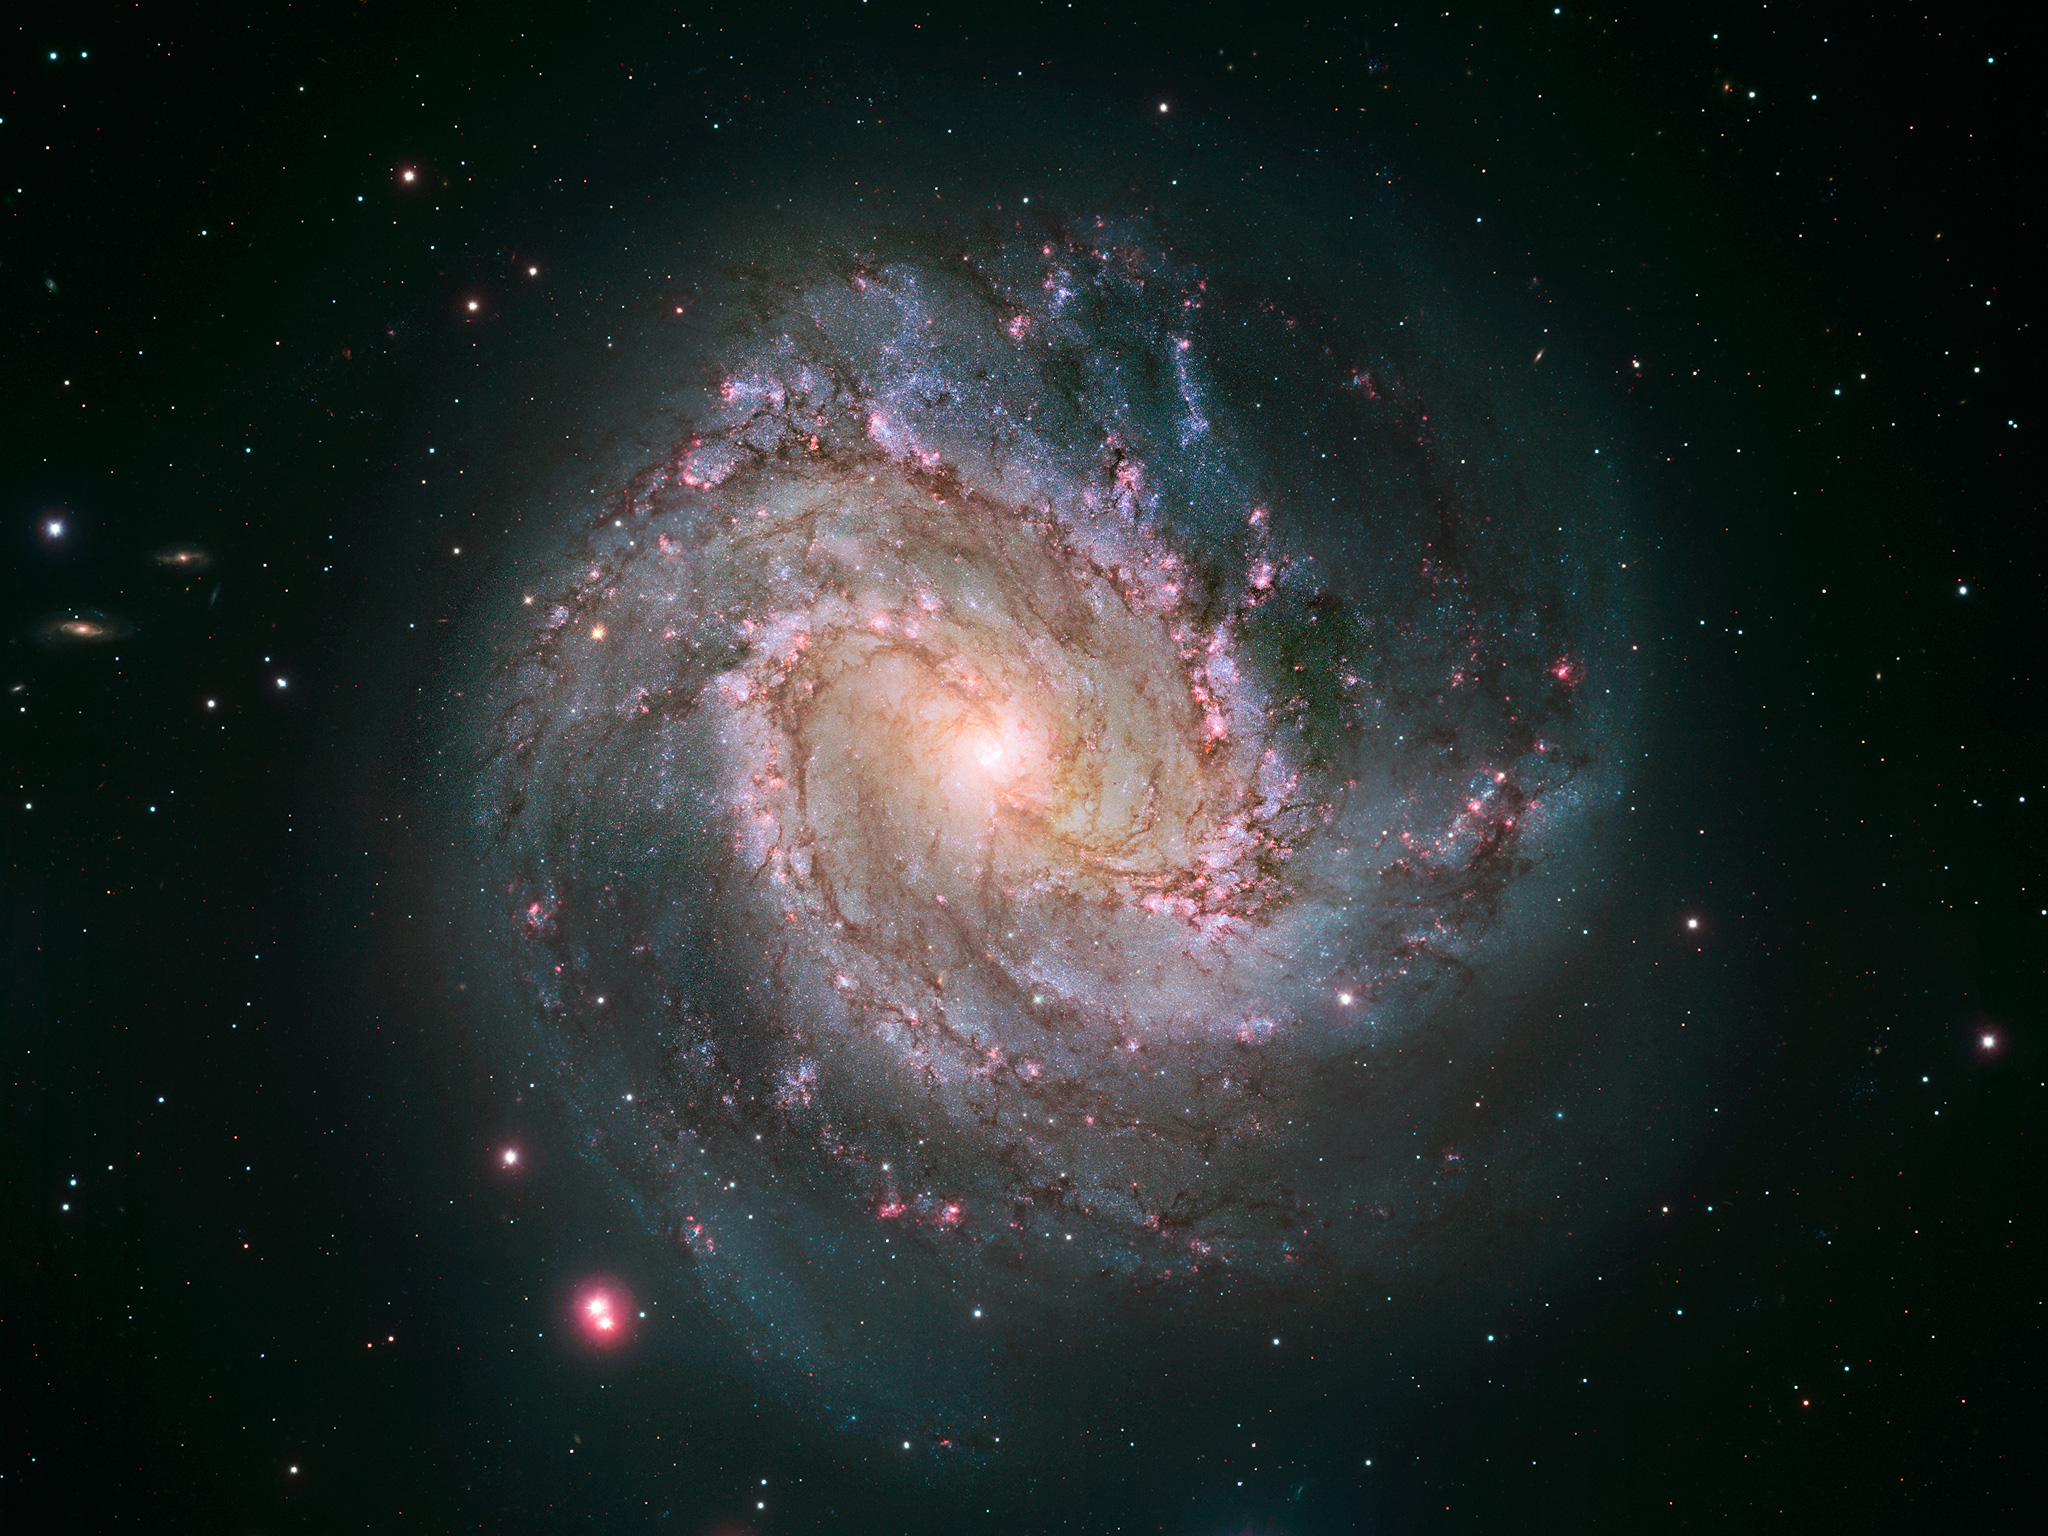
\includegraphics[width=5.64in]{figures/heic1403b.jpg}
\caption{Caption of the image}
\end{figure}
\chapter{Cap\'itulo 3: Contexto. Proyecto}
Lorem ipsum dolor sit amet, consectetur adipiscing elit, sed eiusmod tempor incidunt ut labore et dolore magna aliqua. Ut enim ad minim veniam, quis nostrud exercitation ullamco laboris nisi ut aliquid ex ea commodi consequat. Quis aute iure reprehenderit in voluptate velit esse cillum dolore eu fugiat nulla pariatur. Excepteur sint obcaecat cupiditat non proident, sunt in culpa qui officia deserunt mollit anim id est laborum.

\begin{lstlisting} 
let a = 2;
\end{lstlisting}
 
\chapter{Cap\'itulo 4: Desarrollo}
\section{Primera parte}
\subsection{Estudio previo}
Lorem ipsum dolor sit amet, consectetur adipiscing elit, sed eiusmod tempor incidunt ut labore et dolore magna aliqua. Ut enim ad minim veniam, quis nostrud exercitation ullamco laboris nisi ut aliquid ex ea commodi consequat. Quis aute iure reprehenderit in voluptate velit esse cillum dolore eu fugiat nulla pariatur. Excepteur sint obcaecat cupiditat non proident, sunt in culpa qui officia deserunt mollit anim id est laborum.
 
\chapter{Cap\'itulo 5: Dificultades encontradas}
\section{Problema 1} 

 
\chapter{Cap\'itulo 6: Conclusiones}



\begin{table}[H]
\centering
\begin{tabular}{|p{1.0in}|p{3.2in}|} \hline 
\textbf{Col1} & \textbf{Col2} \\ \hline 
A & 1 \\ \hline 
B & 2 \\ \hline 
C & 3 \\ \hline 
\end{tabular}

\caption[Lo que aparecerá en el listado ]{Caption text}
\label{table:name}
\end{table}

 


 

 
\appendix
\renewcommand\chaptername{Anexo}  
\renewcommand{\thechapter}{\Roman{chapter}}

\noappendicestocpagenum
\appendixpage
\addappheadtotoc
\chapter{Análisis de Impacto}
Reflexión cuantitativa o cualitativamente, sobre el posible impacto (positivo o negativo, directo o indirecto, actual o futuro) y las responsabilidades relacionadas con el TFT:  impacto social: grupos de interés afectados, accesibilidad, seguridad, privacidad, bienestar…  Impacto económico: viabilidad, mejora de la productividad, mantenimiento…  impacto medioambiental: sostenibilidad, consumo energético y otros recursos naturales, contaminación, reciclaje…  responsabilidad ética y profesional: gestión y control de riesgos, respeto a las normas o regulaciones profesionales o legales, respeto a los derechos de propiedad intelectual, respeto a la legislación sobre protección de datos, respeto a los códigos deontológicos de la ingeniería…  
% \addcontentsline{toc} {chapter}{\numberline {}Anexo I}
\chapter{Presupuesto económico}

Presupuesto económico adecuado para un trabajo como el realizado o propuesto en el TFT, cubriendo aspectos como los gastos de ejecución material, los honorarios de los ejecutantes, los impuestos implicados, etc

% \listoftodos


% \appendix
% Reflexión cuantitativa o cualitativamente, sobre el posible impacto (positivo o negativo, directo o indirecto, actual o futuro) y las responsabilidades relacionadas con el TFT:  impacto social: grupos de interés afectados, accesibilidad, seguridad, privacidad, bienestar…  Impacto económico: viabilidad, mejora de la productividad, mantenimiento…  impacto medioambiental: sostenibilidad, consumo energético y otros recursos naturales, contaminación, reciclaje…  responsabilidad ética y profesional: gestión y control de riesgos, respeto a las normas o regulaciones profesionales o legales, respeto a los derechos de propiedad intelectual, respeto a la legislación sobre protección de datos, respeto a los códigos deontológicos de la ingeniería…  
% \appendix

% \addcontentsline{toc} {chapter}{\numberline {}Anexo II}

%Presupuesto económico adecuado para un trabajo como el realizado o propuesto en el TFT, cubriendo aspectos como los gastos de ejecución material, los honorarios de los ejecutantes, los impuestos implicados, etc


%\include{biblio}
\bibliographystyle{unsrt}  
% \bibliographystyle{thesis_style/upmthesis}
\bibliography{thesis}
\addcontentsline{toc} {chapter}{\numberline {}Bibliografía}{}
\end{document}
